\svnkwsave{$RepoFile: elton/blog/KStori.tex $}
\svnidlong {$HeadURL: svn://zero.physics.gatech.edu/elton/blog/KStori.tex $}
{$LastChangedDate: 2015-01-23 18:43:45 -0500 (Fri, 23 Jan 2015) $}
{$LastChangedRevision: 252 $} {$LastChangedBy: predrag $}
\svnid{$Id: KStori.tex 252 2015-01-23 23:43:45Z predrag $}

  \renewcommand{\ssp}{x}            %state space point
  \newcommand{\eps}{\varepsilon}

\chapter{Invariant tori of the Kuramoto-Sivashinsky flow}
%  on Lagrangian mixing}
\label{chap:KStori}

\hfill  Adam Fox and Predrag Cvitanovi\'c


\section{Kuramoto-Sivashinsky flow}
\label{sec:KS}

\subsection{Energy transfer rates}
\label{sec:energy}
% KSe.tex

\PC{this text is clipped and pasted directly from \refref{SCD07}.}
In this section we discuss a set of such physical observables for the
1-$d$ KS invariant under reflections and translations. They offer a
representation of dynamics in which the symmetries are explicitly
quotiented out. We shall use these {observables}
to visualize a set of solutions.

The {space average} of a function $\obser = \obser(\pSpace,t) = \obser(u(x,t))$  on
the interval $L$,
\beq
    \expct{\obser} = \Lint{\pSpace}\, \obser(\pSpace,t)
    \,,
    \label{rpo:spac_ave}
\eeq
is in general time dependent.
Its mean value is given by the {time average}
\beq
\timeAver{\obser}
    =
\lim_{t\rightarrow \infty} \frac{1}{t} \int_0^t \! d\tau \, \expct{\obser}
    =
\lim_{t\rightarrow \infty} \frac{1}{t} \int_0^t \!
    \Lint{\tau}  d\pSpace\, \obser(\pSpace,\tau)
    \,.
\label{rpo:tim_ave}
\eeq
Evaluation of the infinite time average
\refeq{rpo:tim_ave} on a function of a \po\ or \rpo\
$u_p(\pSpace,t)=u_p(\pSpace,t+\period{p})$ requires only a single
$\period{p}$ traversal,
\beq
  \timeAver{\obser}_p = \frac{1}{\period{p}}
    \int_0^{\period{p}} \! d\tau \, \expct{\obser}
\,.
\label{rpo:u-cyc}
\eeq
The time-dependent $L^2$ norm
of $u$,
\beq
    \expctE=
  \Lint{\pSpace}
  V(x,t)=
  \Lint{\pSpace} \frac{u^2}{2}
  \,,
  \label{ksEnergy}
\eeq
has a physical interpretation\rf{ksgreene88} as the average `energy'
density of the flame front.
The energy \refeq{ksEnergy} is intrinsic to the flow,
independent of the particular ODE basis set chosen to
represent the PDE. In the Fourier
space the energy is a diagonalized quadratic norm,
\beq
\expctE
          =  \sum_{k=-\infty}^{\infty} E_k
\,,\qquad
E_k =
    {\textstyle\frac{1}{2}}|a_k|^2
\,,
\ee{EFourier}
and explicitly invariant term by term under translations
% \refeq{eq:shiftFour}
and reflections.
% \refeq{KSparity}.
The energy variation\rf{ksgreene88}
\beq
   \dot{\expctE} = P - D
                \,,\qquad
      P =  \expct{u_{x}{}^2}
                \,,\quad
      D =  \expct{u_{xx}{}^2}
\ee{EnRate}
balances the power $P$ pumped in by anti-diffusion $u_{xx}$
against the energy dissipation rate $D$
by hyper-viscosity $u_{xxxx}$
in the KS equation \refeq{eq:kseq}. %ks}.

The time averaged energy density  $\timeAver{E}$
computed on a typical orbit goes to a constant, so
the expectation values \refeq{rpo:EtimAve} of drive and dissipation
exactly balance each out:
\beq
    \timeAver{\dot{E}}  =
    \lim_{t\rightarrow \infty}
        \frac{1}{t} \int_0^t d\tau \, \dot{\expctE}
=
      \timeAver{P} - \timeAver{D}
= 0
    \,.
\ee{rpo:EtimAve}
In particular, the \eqva\
and \reqva\ fall onto the diagonal in a $[D,P]$
plot, %\reffig{f:drivedrag},
and so do time averages computed on \po s and \rpo s:
\beq
\timeAver{E}_p =
\frac{1}{\period{p}} \int_0^\period{p}d\tau \, E(\tau)
    \,,\qquad
\timeAver{P}_p =
\frac{1}{\period{p}} \int_0^\period{p} d\tau \, P(\tau)
    =
      \timeAver{D}_p
    \,.
\label{poE}
\eeq
In the Fourier basis \refeq{EFourier} the conservation of energy on average
takes form
\beq
0 = \sum_{k=-\infty}^{\infty} ( q_k^2 - q_k^4 )\,
    \timeAver{E}_k
\,,\qquad
E_k(t) =  {\textstyle\frac{1}{2}} |a_k(t)|^2
\,.
\ee{EFourier1}
The large $k$ convergence of this series is insensitive to the
system size $L$; $\timeAver{E_k}$ have to decrease much faster than
$q_k^{-4}$.
Deviation of $E_k$ from this bound for small $k$ determines the active modes.


\subsection{An invariant torus of the Kuramoto-Sivashinsky flow}
\label{sec:KStori}


%%%%%%%%%%%%% back to Adam %%%%%%%%%%%%%%%%%%%%%%%%%%%%%%%%%%%%%%

I am following Lan's example, computing tori on the $a_1=0.06$ Poincar\'e
section, and allowing the rotation number $\omega$ to be fixed by the
geometry.  I began by using Lan's initial condition at $L=40.95$ and
computed the torus up to an accuracy of $10^{-4}$.  Once computed, I used
this value as an initial condition for the torus at $L=L+0.01$.  I
repeated this process until the algorithm failed to converge to the
specified tolerance.  I then repeated, however went in the opposite
direction (ie, I set $L=L-0.01$).  I was able to compute tori for $L\in
[40.81,41.34]$.  These tori are initially large, and contract to a
\po\ at the upper critical system size $L=40.85$, as seen in the plot below.  The rotation number
$\omega$ appears to change smoothly with $L$, also shown below.

\begin{figure}%[H]
\centering
 (a) 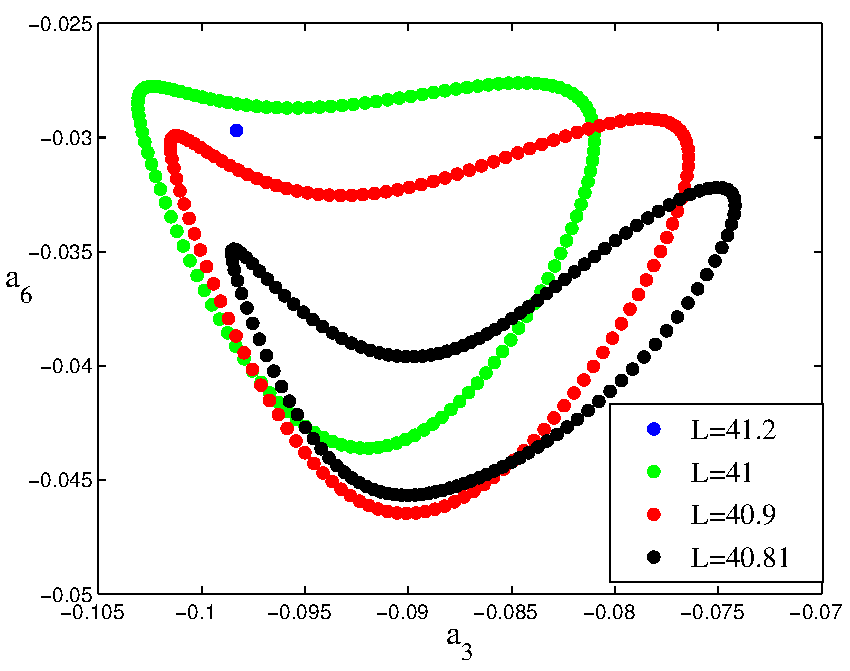
\includegraphics[width=0.45\textwidth]{KSTori.pdf}
 (b) 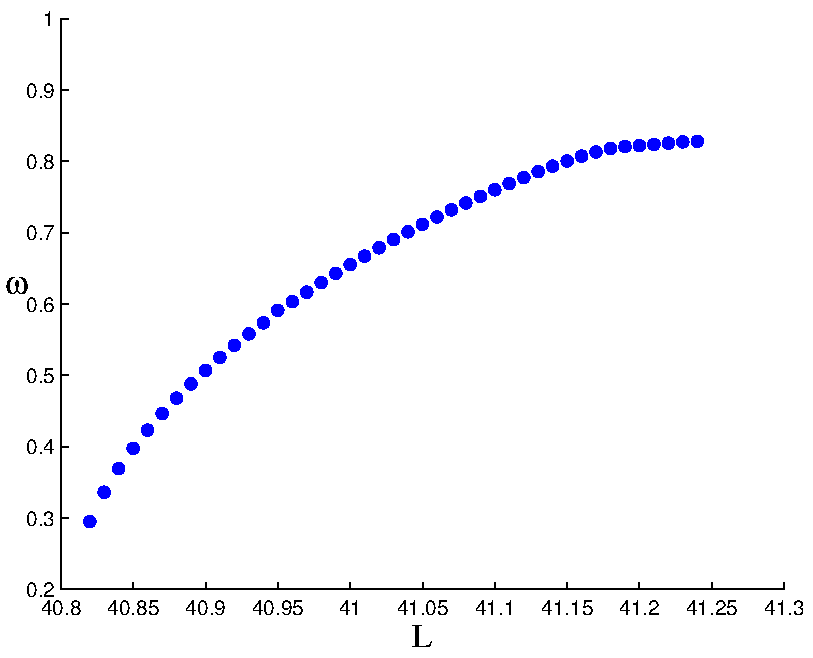
\includegraphics[width=0.45\textwidth]{KSRotNum.pdf}
\caption{
(a)
Projection of the torus Poincar\'e sections for a family of
\KS\ systems with $L \in [40.81,41.34]$.
(b)
Rotation number of the tori as a function of $L$.
}
\label{fig:PsecTorus}
\end{figure}

I also attempted to find tori with fixed $\omega$.  This did not work -  I believe $\omega$ must be fixed by the geometry.  This may imply that there are not families of tori, but only a few (or perhaps even one).
